\section{Design Document}
\subsection{High Level Architecture}

In the application, client-server architecture is being used.\\ \\

The server side is built with Django version 1.10.3. Due to frequent 
changes in the django environment, sticking to this version is advised
for further development. Django API along with "networks" library
in python is responsible for making calls to USDA service. The USDA 
service has a API limit. To leverage that, the system includes an 
internal cache database that's on the same level with the USDA application which caches the queries, and the results of the queries
in the system so that when a query is remade, it will be ready to use
in our database. This behaviour will make better use when users are searching for food with few letters only.

The client side is built with HTML, CSS and JavaScript. In the development, some frequently used components are used, Namely Bootstrap,
bootstrap.js and jquery. Their use has been mostly to validate 
user inputs on forms like registration, search etc.

As a database, there's no restriction, however, for ease of use SQLite
is recommended and is used in initial deployment as Django handles it.

In this system's design, cookies and browser caches are not used,
not depended on.

\subsection{Behavioural and Functional Design}

In this section, processes will be explained with sequence diagrams.


\newpage
\subsubsection{Sign-up Process}
\begin{figure}[H]
\centering
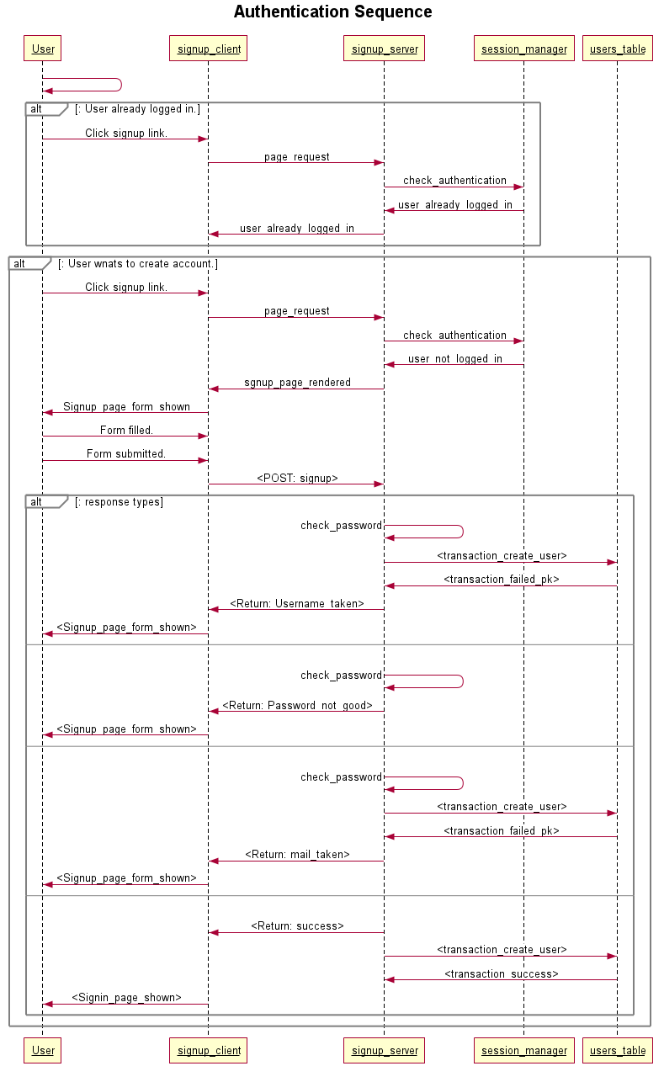
\includegraphics[scale=0.70]{signup}
\end{figure}

\newpage
\subsubsection{Sign-in Process}
\begin{figure}[H]
\centering
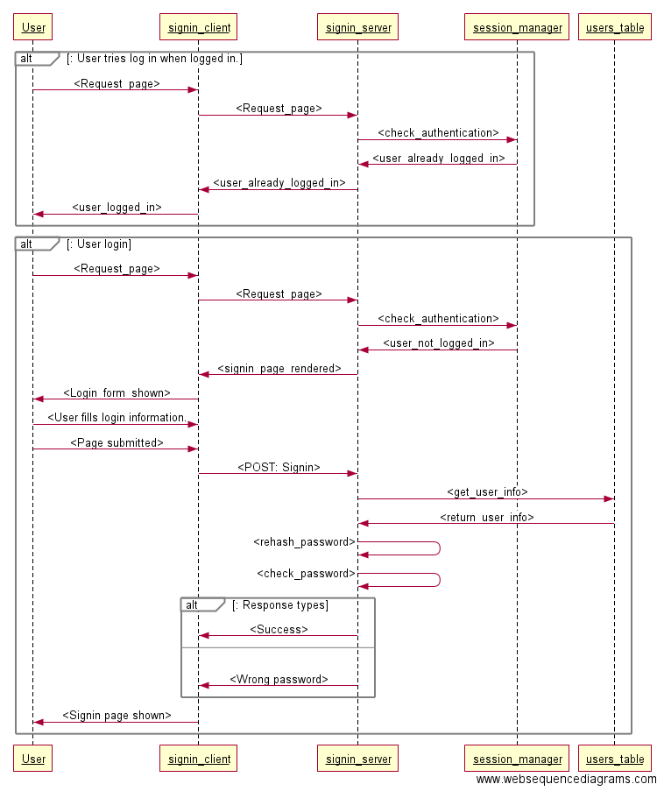
\includegraphics[scale=0.70]{signin}
\end{figure}


\newpage
\subsubsection{Food Search Process}
\begin{figure}[H]
\centering
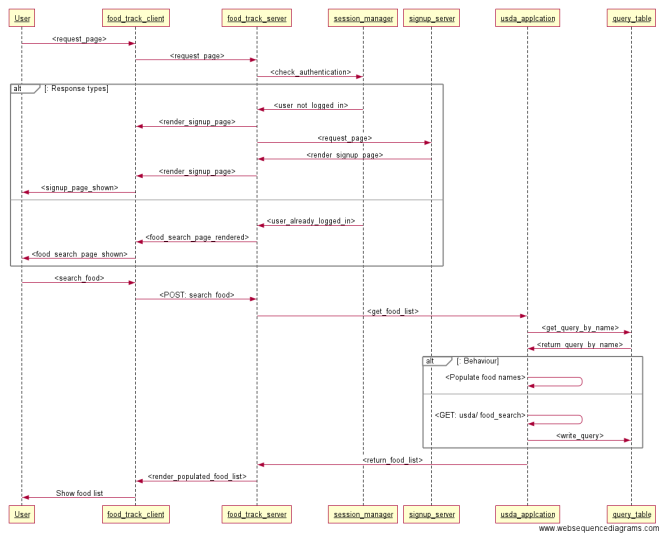
\includegraphics[scale=0.70]{search_food}
\end{figure}



\newpage
\subsubsection{Activity Search and Tracking Process}
\begin{figure}[H]
\centering
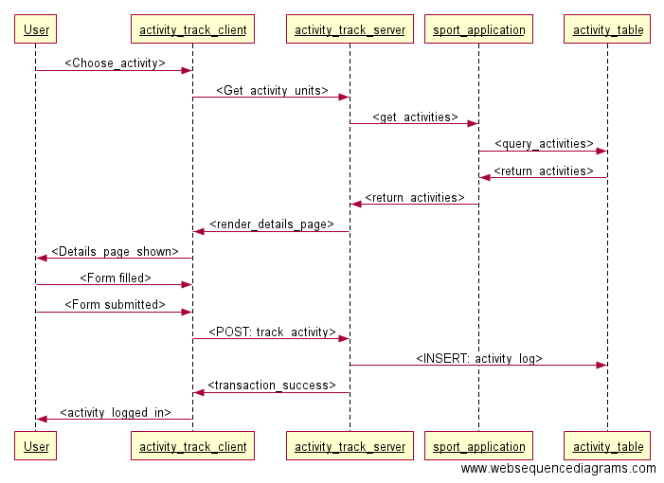
\includegraphics[scale=0.70]{activity}
\end{figure}



\newpage
\subsubsection{Food Tracking Process}
\begin{figure}[H]
\centering
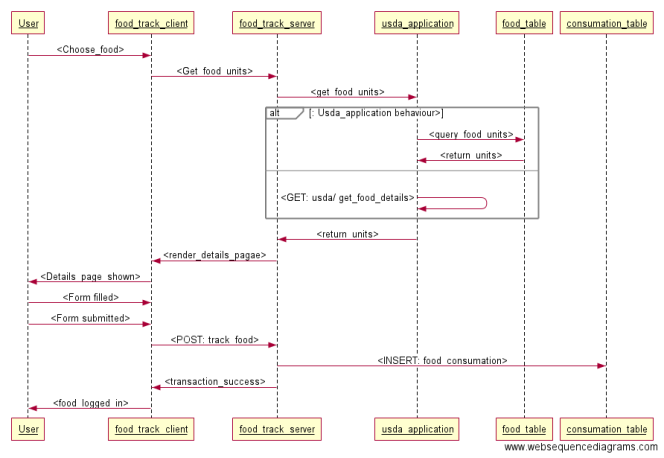
\includegraphics[scale=0.70]{consumation}
\end{figure}